\section{Solving the Vehicle Routing Problem with Time Windows (VRPTW) Using Ant Colony Optimization (ACO) and Particle Swarm Optimization (PSO)}
This task focuses on optimizing the delivery routes for a fleet of vehicles using two nature inspired optimization algorithms: Ant Colony Optimization (ACO) and Particle Swarm Optimization (PSO). 
\newline
We defined the objective is to find the most efficient routes for a set of vehicles, that all customers receive their deliveries within specified time windows. 
\newline
We have implemented both Ant Colony Optimization, and Particle Swarm Optimization to solve the Vehicle Routing Problem with Time Windows. Then we compared the effectiveness of these algorithms. 
\newline
\subsection{Data Exploration, and pre processing}
We have used Solomon’s VRPTW Benchmark Problems dataset, C101.txt.[5]
\newline
The columns dataset are:
\newline
CUST NO.: Customer number (ID).
\newline
XCOORD: X coordinate of the customer's location.
\newline
YCOORD: Y coordinate of the customer's location.
\newline
DEMAND: The demand at the customer location.
\newline
READY TIME: The earliest time at which service can begin DUE DATE: The latest time by which the service should be completed.
\newline
SERVICE TIME: The time it takes to complete the service for this customer.
\newline
\begin{figure}[h]
    \centering
    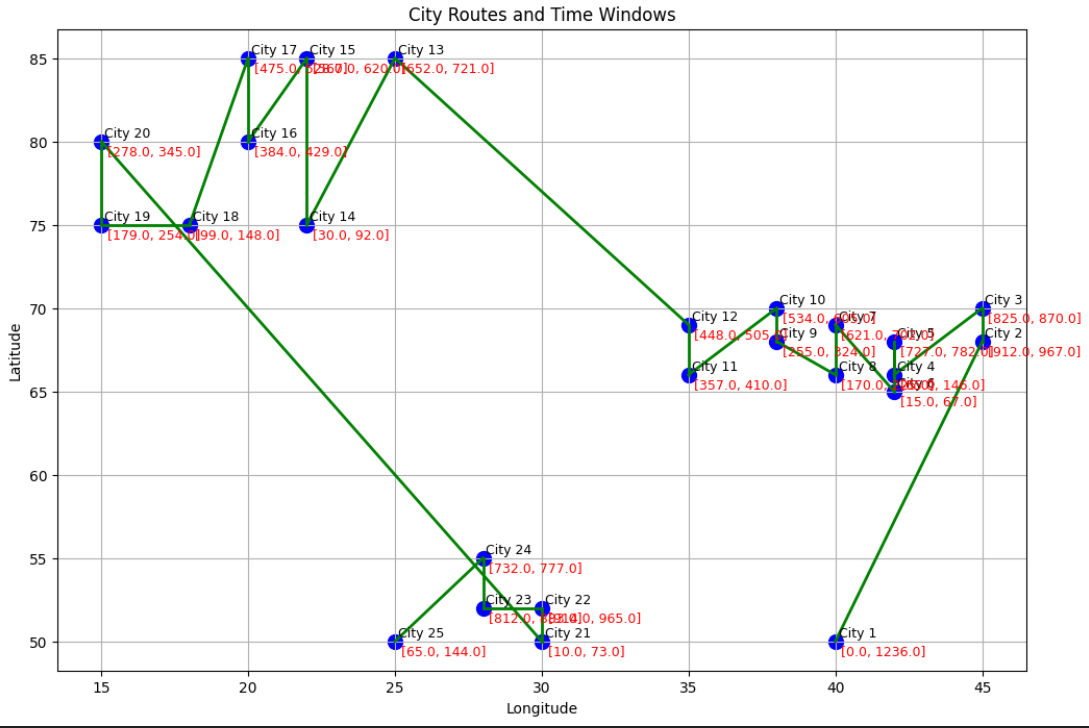
\includegraphics[width=1\linewidth]{figures/Citye_Routes_And_Time_Windows.PNG}
    \caption{City Routes And Time Windows}
    \label{fig:PSO Algorithms Analyse}
\end{figure}
\subsection{Problem Formulation}
\subsubsection{A. Define the VRPTW for the chosen dataset}
\subsubsection{B. Formulate the objective function that minimizes total travel distance while 
penalizing violations of time windows}
\subsection{Algorithm Implementation}
\subsubsection{A. Implement ACO}
\subsubsection{B. Implement PSO}
\subsubsection{Incorporate heuristic and penalty mechanisms }
\subsection{Performance Evaluation}
\subsubsection{Results}
\begin{figure}[h]
    \centering
    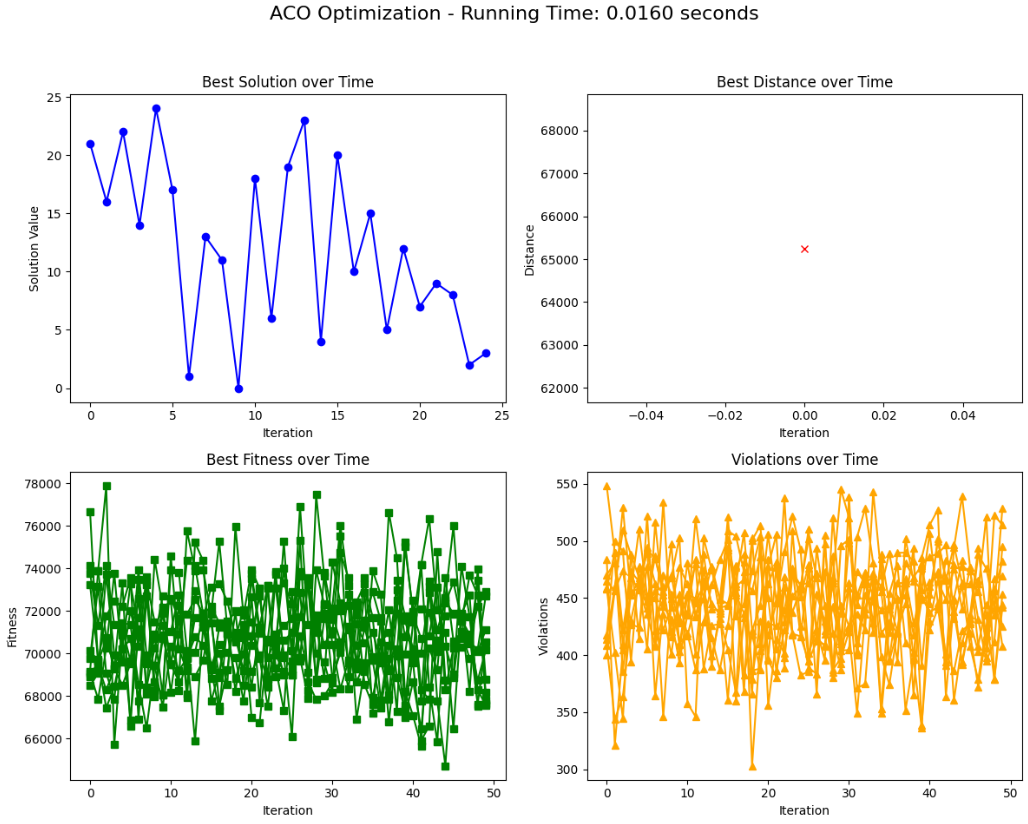
\includegraphics[width=1\linewidth]{figures/Aco_Results.PNG}
    \caption{ACO Algorithms Analyse}
    \label{fig:ACO Algorithms Analyse}
\end{figure}
\begin{figure}[h]
    \centering
    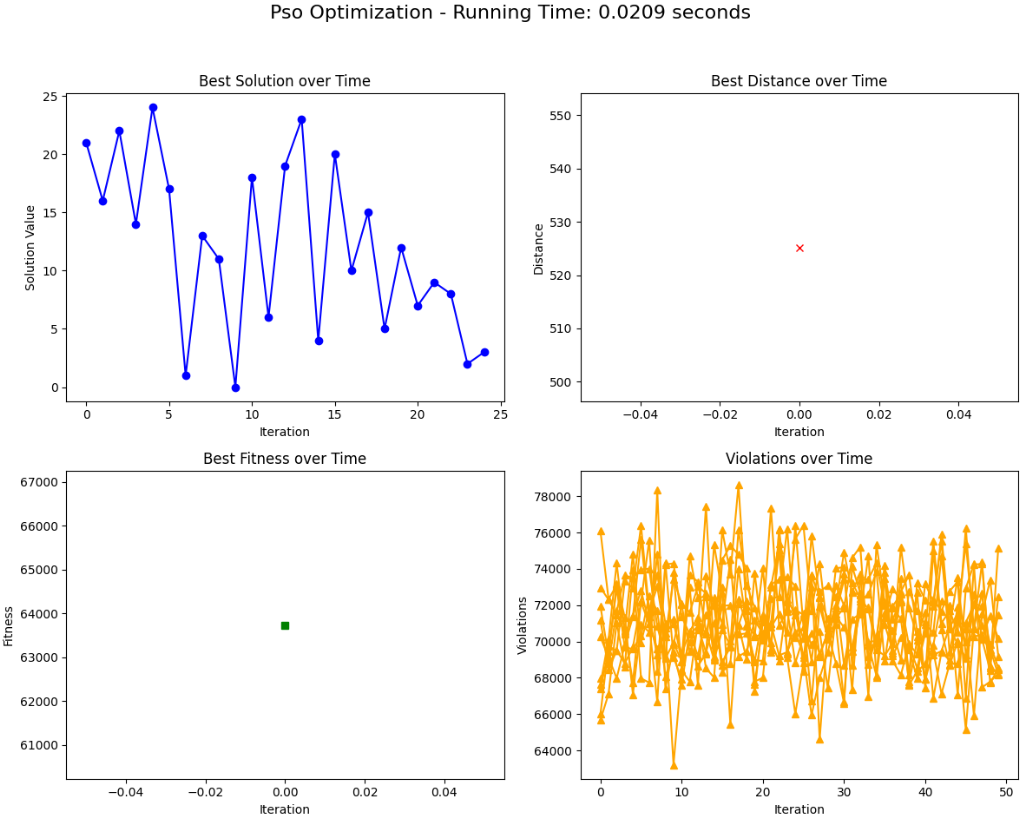
\includegraphics[width=1\linewidth]{figures/Pso_Results.PNG}
    \caption{PSO Algorithms Analyse}
    \label{fig:PSO Algorithms Analyse}
\end{figure}



